\section{Preliminarii}

\subsection{Elemente de teorie muzicală}
\noindent
Pentru a prezenta funcționalitățiile aplicației este necesară definirea câtorva termeni care descriu aspecte fundamentale ale melodiei. 

\subsubsection{Armonie}
\noindent Armonia reprezintă procesul prin care sunete individuale sunt aranjate în unități individuale. Fiecare notă muzicală are asociată o anumită frecvență, reprezentând numărul de oscilații produse într-o secundă de semnalul sonor obținut prin redarea sa. Raportul dintre frecvența a două note muzicale corespunde nivelului de \textit{consonanță} dintre cele două. Consonanța este atât un criteriu fizic cât și un fenomen psihologic: două note sunt considerate consonante dacaă redate împreuna formează un sunet plăcut. Astfel, o secvență muzicală este considerată \textit{armonioasă} dacă notele muzicale din care este compusă sunt consonante. \par
\noindent \textbf{Gamă} \par
\noindent Intervalul cuprins între două note cu rația frecvențelor de $2:1$ corespunde unei \textit{octave} și reprezintă baza din care se construiește fiecare \textit{gamă muzicală}. Astfel, problema construcției unei game reprezintă găsirea unei mulțimi de note consonante în acest interval \cite{history}.  În general, compozițiile muzicale sunt scrise folosind predominant note aparținând unei singure game pentru a asigura caracterul armonios. Gamele muzicale pot fi clasificate în funcție de numărul de note: 

\begin{itemize}[topsep=5pt,itemsep=2pt,parsep=0pt,partopsep=0pt]
    \item \textbf{Cromatic, sau dodecatonic} - 12 note
    \item \textbf{Nonatonic} - 9 note
    \item \textbf{Octatonic} - 8 note
    \item \textbf{Heptatonic} - 7 note
    \item \textbf{Hexatonic} - 6 note, etc.
\end{itemize} 

\begin{figure}[H]
    \centering
    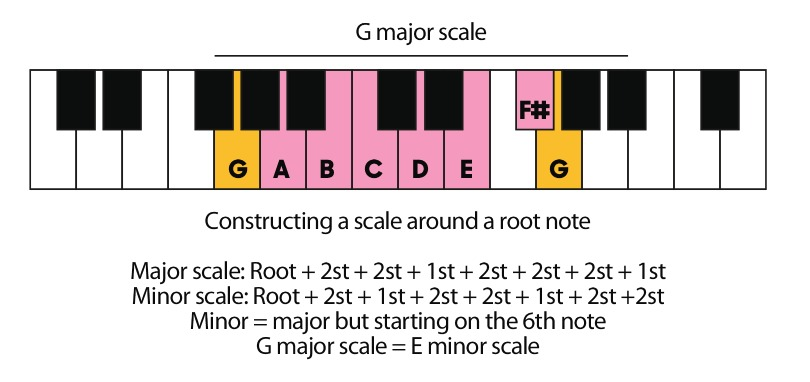
\includegraphics[scale=0.45]{images/scale.jpeg}
    \caption{Construirea unei game în jurul unei note}
    \label{image.scale}
\end{figure}

\noindent \textbf{Mod} \par
\noindent Există mai multe \textit{moduri} în care poate fi construită o gamă, în funcție distanța în frecvență dintre note. Această distanță se calculată în \textit{tonuri (t)} și \textit{semitonuri (s)}. În continuare, voi utiliza doar game heptatonice în următoarele moduri:

\begin{itemize}[topsep=0pt,itemsep=0pt,parsep=0pt,partopsep=0pt]
    \item \textbf{Aeolian (minor)}: t-s-t-t-s-t-t
    \item \textbf{Locrian}: s-t-t-s-t-t-t
    \item \textbf{Ionian: (major)} t-t-s-t-t-t-s
    \item \textbf{Dorian}: t-s-t-t-t-s-t
    \item \textbf{Phrygian}: s-t-t-t-s-t-t
    \item \textbf{Lydian}: t-t-t-s-t-t-s
    \item \textbf{Mixolydian}: t-t-s-t-t-s-t
\end{itemize}

\noindent \textbf{Acord} \par
\noindent Un acord este o combinație de note consonante redate simultan. Cele mai întâlnite acorduri sunt triadele, compuse din 3 note aparținând aceleiași game muzicale.  \par

\begin{table}[H]
    \begin{center}

    \begin{tabular}{ c c c }
        \hline
        Acord & Note & Notație \\
        \hline
        1 & G B D & I \\
        2 & A C E & ii \\
        3 & B D F\# & iii \\
        4 & C E G & IV \\
        5 & D F\# A & V \\
        6 & E G B & vi \\
        7 & F\# A C & vii \\
        \hline
    \end{tabular}
    \caption{Triadele diatonice în G major}
    \end{center}
\end{table}

\noindent O înșiruire de acorduri se numește progresie de acorduri. În general, progresiile de acorduri reprezintă fundația armoniei într-o piesă muzicală.

\subsubsection{Ritm}

\noindent Ritmul reprezintă alternarea recurentă și simetrică între elemente distincte. Ticurile unui ceas sunt un exemplu concret de ritm. Ticurile ceasului sunt evenimente despărțite în timpi egali și sunt percepute diferit (tic-tac), deși sunt identice. Gruparea impulsurilor (tic-tac) formează nivele noi de periodicitate, care compun o structura pe mai multe nivele, numită \textit{metru}. 

\begin{figure}[H]
    \centering
    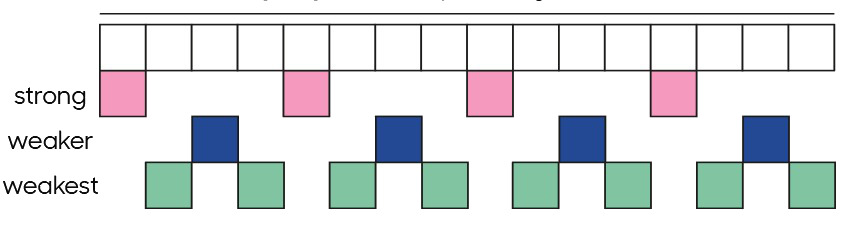
\includegraphics[scale=1.8]{images/rhythm.jpeg}
    \caption{Exemplu de metru}
    \label{image.rhythm}
\end{figure}

Alternarea periodică între \textit{impulsuri (beats) puternice} și \textit{impulsuri slabe} slabe este fundamentală pentru ideea de metru \cite{lerd}. Impulsurile puternice nu diferă într-un sens fizic (e.g. frecvență, durată, amplitudine) de cele slabe, dar sunt percepute ca fiind fundamentale. Gruparea pulsurilor in grupuri cu număr non-prim de elemente pot fi subdivizate in subgrupuri de pulsuri egale ca dimensiune. Astfel, se crează o structură metrică pe mai multe nivele \cite{sync}. În figura 2.2 sunt ilustrate nivelele metrice ale unei grupări cu 4 elemente. Pulsurile marcate cu roz se numesc \textit{downbeats}, cele marcate cu verde \textit{upbeats}, iar cele verzi \textit{backbeats}. \par
\noindent \textbf{Notă} \\
\noindent În teoria muzicală vestică, un eveniment sonor este denumit \textit{notă}, în timp ce un eveniment silențios este numit \textit{pauză}. Fiecărei note sau pauze îi este asociată o \textit{durată (sau valoare)}. Valorile notelor nu reprezintă unități absolute de timp, ci sunt definite relativ la nota întreagă. Notele pot fi acompaniate de diferite \textit{accente}, care modifică durata, frecvența(tonalitatea) sau intensitatea. \par

\begin{table}[H]
    \begin{center}
    \renewcommand{\arraystretch}{1.5}
    \begin{tabular}{ c c c c }
         \hline
         \\[-3.8em]
         Notă & Pauză & Valoarea notei & Denumire \\
         \hline
         \Large \wholeNote & \large \wholeNoteRest  & $1$ & Notă întreagă \\  
         \large \halfNote & \large \halfNoteRest & $\frac{1}{2}$ & Doime \\
         \large \crotchet & \large \crotchetRest & $\frac{1}{4}$ & Pătrime \\
         \large \quaver & \large \quaverRest & $\frac{1}{8}$ & Optime\\
         \large \semiquaver & \large \semiquaverRest & $\frac{1}{16}$ & Şaisprezecime \\
         \hline
    \end{tabular}
    \caption{Durata notelor muzicale}
    \end{center}
\end{table}

\noindent O secvență de note poate fi sincronizată cu structura metrică, caz în care aceasta devine o unitate ritmică. Există mai multe moduri prin care se poate realiza sincronizarea: \cite{rhythm}

\begin{itemize}[topsep=0pt,itemsep=0pt,parsep=0pt,partopsep=0pt]
    \item \textbf{Metric}: Valorile notelor sunt identice cu pulsurile unui nivel metric.
    \item \textbf{Intrametric}: Valorile notelor sunt bazate pe grupări de pulsuri din structura metrică dar nu sunt egale cu pulsurile din structura metrică, însă accentele lor corespund accentuării din structura metrică.
    \item \textbf{Contrametric}: Valorile notelor sunt identice cu pulsurile unui nivel metric sau sunt bazate pe grupări de pulsuri din structura metrică dar accentele lor nu corespund accentuării din structura metrică, ci o perturbă.
    \item \textbf{Extrametric}: Valorile notelor sunt bazate pe grupări de pulsuri din afara structurii metrice.
\end{itemize}

\subsubsection{Compoziție}
\noindent Structura unei secvențe muzicale diferă în funcție de instrumentul pentru care aceasta este compusă. Instrumentele muzicale pot fi \textit{monofonice} (o singură notă este redată în orice moment) sau \textit{polifonice} (mai multe note pot fi redate simultan). În funcție de rolul lor în compoziție, instrumentele pot fi încadrate în mai multe categorii, printre care: \par

\begin{itemize}
    \item \textbf{Bass:} monofonic, redă note cu frecvențe reduse (până în ~260Hz) 
    \item \textbf{Lead:} monofonic, este compus din note cu frecvențe mijlocii sau ridicate și are rolul de a reda melodia
    \item \textbf{Pad:} polifonic, este ambiental și are rolul de a stabili armonia
\end{itemize}

\subsection{Metode de măsurare a nivelului de sincopare}
\noindent Sincopa este contradicția monentană a structurii ritmice predominante i.e. o secvență de note este sincopată atunci cānd sincronizarea sa cu structura ritmică se realizează în mod contrametric \cite{rhythm}. Pentru a ilustra modul de calculare al metodelor prezentate voi folosi secvența "Bossa-Nova".

\begin{figure}[H]
    \centering
    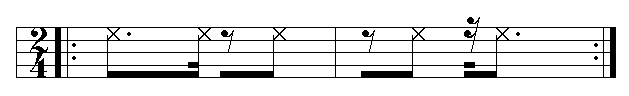
\includegraphics{images/bossa_nova.png}
    \caption{Bossa nova}
    \label{fig:bossa}
\end{figure}

\subsubsection{Gómez "Weighted Note-to-Beat"}
\label{wnbd}
\noindent Modelul "Weighted Note-to-Beat" \cite{Gomez} definește nivelul de sincopare al unei note ca fiind distanța dintre pulsurile metrului. Pentru a calcula distanța $D_{WNBD}(S)$ definim întâi $x_n$ o notă cu $x_n^s$ și $x_n^e$ începutul, respectiv sfărșitul, ${b_i}$, $b_{i+1}$ "beat-urile" între care se află, și distanța $d$.
\begin{equation}
    b_i \leq x_n^s \leq b_{i+1}
\end{equation}
\begin{equation}
    d(x_n, b_i) = \frac{x_n^s - b_i}{b_{i+1}-b_i}
\end{equation}
În continuare definim $T(x_n)$ ca fiind distanța dintre ${x_n}$ și cel mai apropiat beat.
\begin{equation}
    T(x_n) = min(d(x_n, b_i), d(x_n, b_{i+1}))
\end{equation}
Valoarea $W(x_n)$ reprezintă nivelul de sincopare al unei note și se calculează astfel:
\begin{equation}
    W(x_n) = 
    \begin{cases}
        \hfil 0, & \text{dacă } d(x_n, b_i) = 0 \\
        \frac{2}{T(x_n)}, & \text{dacă } b_{i+1} < x_n^e \leq b_{i+2} \\
        \frac{1}{T(x_n)}, & \text{altfel}
    \end{cases}
\end{equation}
În final, nivelul de sincopare al unei structuri ritmice se calculează astfel:
\begin{equation}
    D_{WNBD}(S) = \frac{1}{|Y|}\sum_{n=0}^{|Y|-1}{W(x_n)}
\end{equation}

Spre exemplu, pentru secvența Bossa-Nova ponderile notelor sunt (0, 4, 8, 8, 4), deci WNBD prezice un nivel de sincopare de valoare 3.

\subsubsection{Toussaint "Off-Beatness"}
\label{ob}
\noindent Modelul "Off-Beatness" \cite{Toussaint} definește o notă ca fiind sincopată atunci câ este redată în timpul unui puls "off-beat". Un puls este considerat off-beat dacă începe în același timp cu un puls din mulțimea formată din generatorii grupului ciclic $C_{n}$, unde $n$ este numărul de pulsuri al metrului. Pentru a calcula nivelul de sincopare $D_{TOB}$ al unei structuri ritmice definim întâi $B$ ca fiind mulțimea numerelor non-prime față de $n$ .
\begin{equation}
    B = \{i, \: n \text{ mod } i = 0 : 1 < i < n\}
\end{equation}
Valoarea $W(x_n)$ reprezintă nivelul de sincopare al unei note și se calculează astfel:
\begin{equation}
    W(x_n) = 
    \begin{cases}
        0, & \text{dacă $x$ mod } i = 0 \: \forall \: i \in B\\
        1, & \text{altfel}
    \end{cases}
\end{equation}
În final, nivelul de sincopare al unei structuri ritmice se calculează folosind modelul "Off-Beatness" astfel:
\begin{equation}
    D_{TOB}(S) = \frac{1}{|Y|}\sum_{n=0}^{|Y|-1}{W(x_n)}
\end{equation}
Pentru secvența Bossa-Nova conține 16 pulsuri, iar notele sunt distribuite astfel: [x..x..x...x..x..]. Așadar, a 2-a și a 5-a sunt offbeat, deci nivelul de sincopare prezis este 2.

\subsection{Formatul MIDI}
\noindent Formatul MIDI (Musical Instrument Digital Interface) este un standard tehnic care descrie un protocol de comunicații, o interfață digitală și tipuri de conectori electrici care conectează instrumente muzicale electronice și dispozitive audio. Informația MIDI este transmisă prin \textit{mesaje MIDI}. Acestea sunt formate dintr-un \textit{status byte}, urmat de unul sau mai mulți \textit{data bytes} și pot fi clasificate drept "System Messages, "Channel Voice Messages" și "channel mode messages". \cite{midi} \par
\noindent \textbf{Channel Voice Messages} \par 
\noindent Channel Voice Messages sunt folosite pentru a transmite informații legate de performanța muzicală și sunt de tipul \textit{Note On, Note Off, Polyphonic Key Pressure, Channel Pressure, Pitch Bend Change, Program Change}, sau \textit{Control Change messages}. O notă muzicală este transmisă pentru a fi redată folosind un mesaj de tipul Note On, indicāndu-se nota (tonică) și velocitatea, urmat de un mesaj de tipul Note Off. Astfel, durata notei este calculată în funcție de diferența dintre timpii la care s-au primit cele 2 evenimente. \par
\noindent \textbf{Channel Mode Messages} \par
\noindent Channel Mode Messages afectează modul în care sintetizatoarele răspund datelor MIDI. Acestea pot fi folosite pentru Acestea pot fi folosite pentru a selecte între a reda note monofonic sau polifonic.\par
\noindent \textbf{System Messages} \par
\noindent System Messages diferă de celelalte două tipuri prin faptul că nu sunt specifice unui singur canal, deci nu includ un număr de canal în status byte. Acestea pot fi folosite pentru a sincroniza instrumente, sau pentru a transmite mesaje definite exclusiv pentru anumite echipamente.
\noindent \par

\subsection{Audio plugin}

\noindent Un plugin audio este un plugin folosit pentru a adăuga sau îmbunătății funcționalități audio într-un program, în general un DAW (Digital Audio Workstation). Există mai multe arhitecturi care funcționează diferit în funcție de sistemul de operare sau DAW, cele mai utilizate fiind: \par
\begin{itemize}
    \item \textbf{VST (Virtual Studio Technology):} cel mai utilizat format, cross-platform
    
    \item \textbf{AU (AudioUnits):} creat de Apple special pentru MacOS
\end{itemize}
\noindent \textbf{JUCE} \par
\noindent JUCE este un framework de C++ cross-platform folosit pentru a crea audio plugins. Acesta implementează multiple funcționalități audio și oferă posibilitatea exportării proiectelor în majoritatea formatelor.